\begin{figure}[tb]
	\centering
	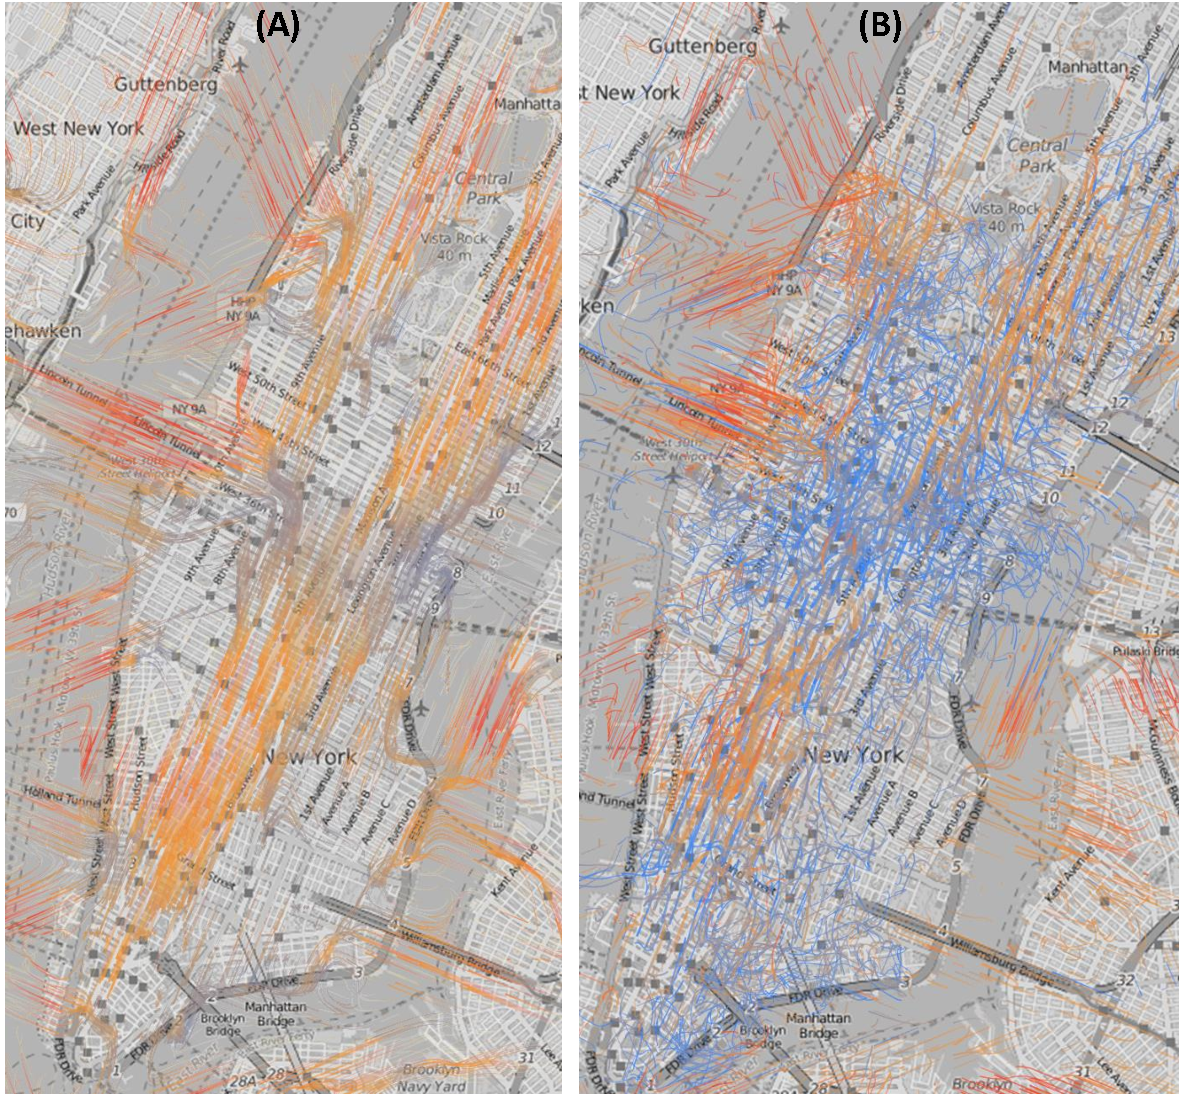
\includegraphics[width=1.0\columnwidth]{twitter_flow}
	\caption{The Major (A) and probability flows (B) of Twitter data between 6:00 AM and 10:00 AM. Note that the probability of a path is accumulated multiplicationaly from the particle birth, the probability in the probability flows might be different from one in the major flows.}
	\label{fig:twitter_flow}
	%\vspace{-0.7cm}
\end{figure}

\begin{figure}[tb]
	\centering
	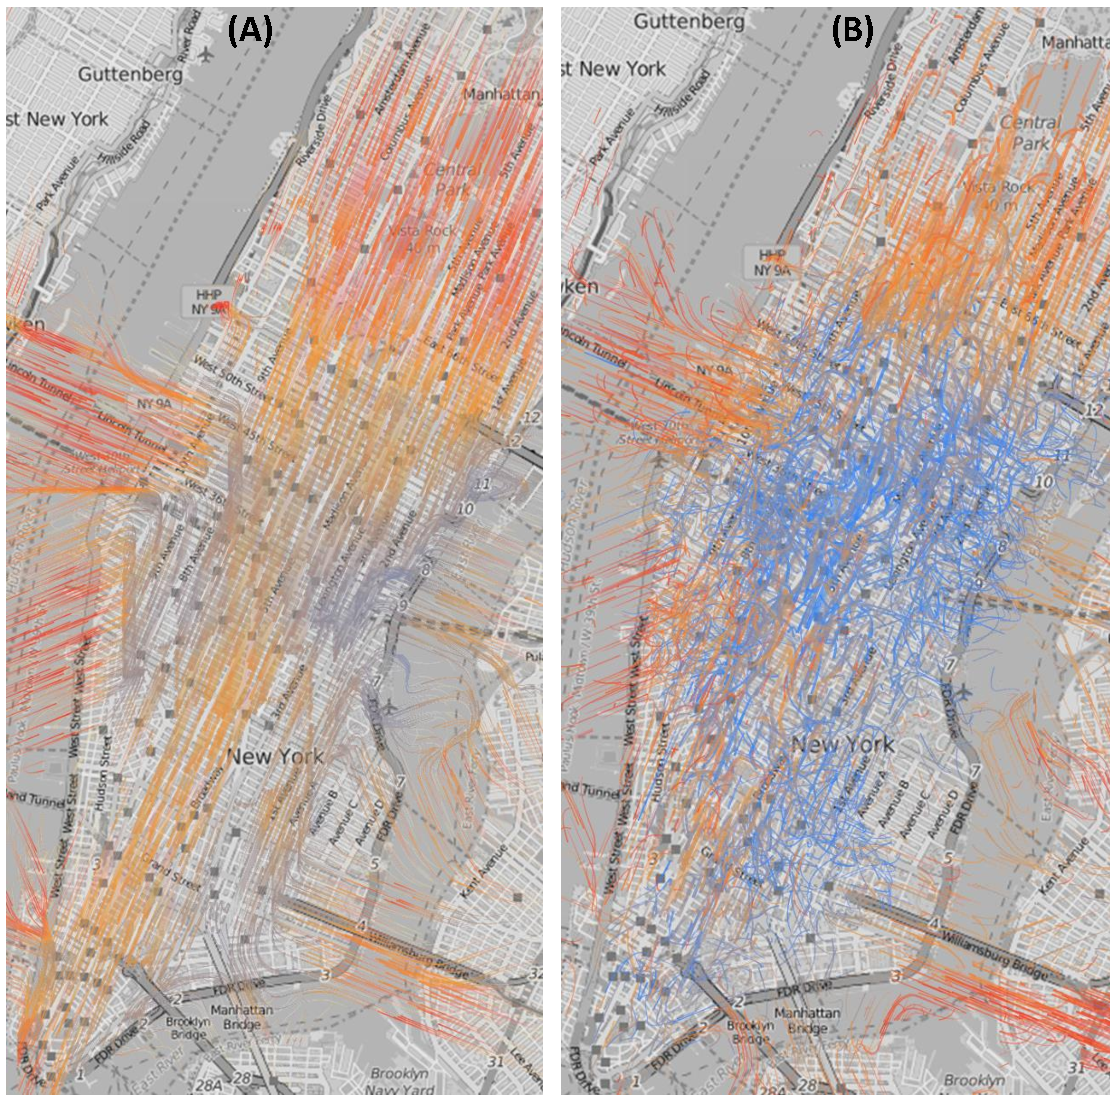
\includegraphics[width=0.93\columnwidth]{twitter_flow_prediction}
	\caption{Forecast Result: The Major (A) and probability flows (B) of Twitter data between 6:00 AM and 10:00 AM. }
	\label{fig:twitter_flow_prediction}
	%\vspace{-0.7cm}
\end{figure}


\subsection{Visualization of Multi-Vector Fields}
\label{sec:forecasting-visualization}

The flow of human crowds represents the temporal trend of human movement within a certain time period. 
Our system is built on several vector field visualization techniques on the generated multi-vector field data in order to observe the trends and patterns. 
%Since we extract the trajectory vector fields, it is possible to apply vector field visualization techniques to observe the trend patterns. 
In this work, we utilize the particle advection technique~\cite{Kruger:FLOW:2005} for the vector fields and extend the web based project, {\textit{earth}}, that visualizes global weather conditions~\cite{earth:2015:online}. 
%
Our web-based flow visualization system consists of JavaScript and several APIs, such as \textit{D3.js}, \textit{Backbone.js}, and \textit{When.js}. The web server visualizes the 3D~globe on the web based according to the vector fields using D3 projections. The server, then, attaches some minimum geographical information including roads, country boundaries, and lakes using the \textit{TopoJSON}. The web-based flow visualization provides animated particles and the color of a particle varies accordingly as the particle ages. If the target vector field area is too small to be visible, our system allows users to apply an additional map of the different map layer located between the globe layer and the particle layer.


\begin{figure*}[tb]
	\centering
	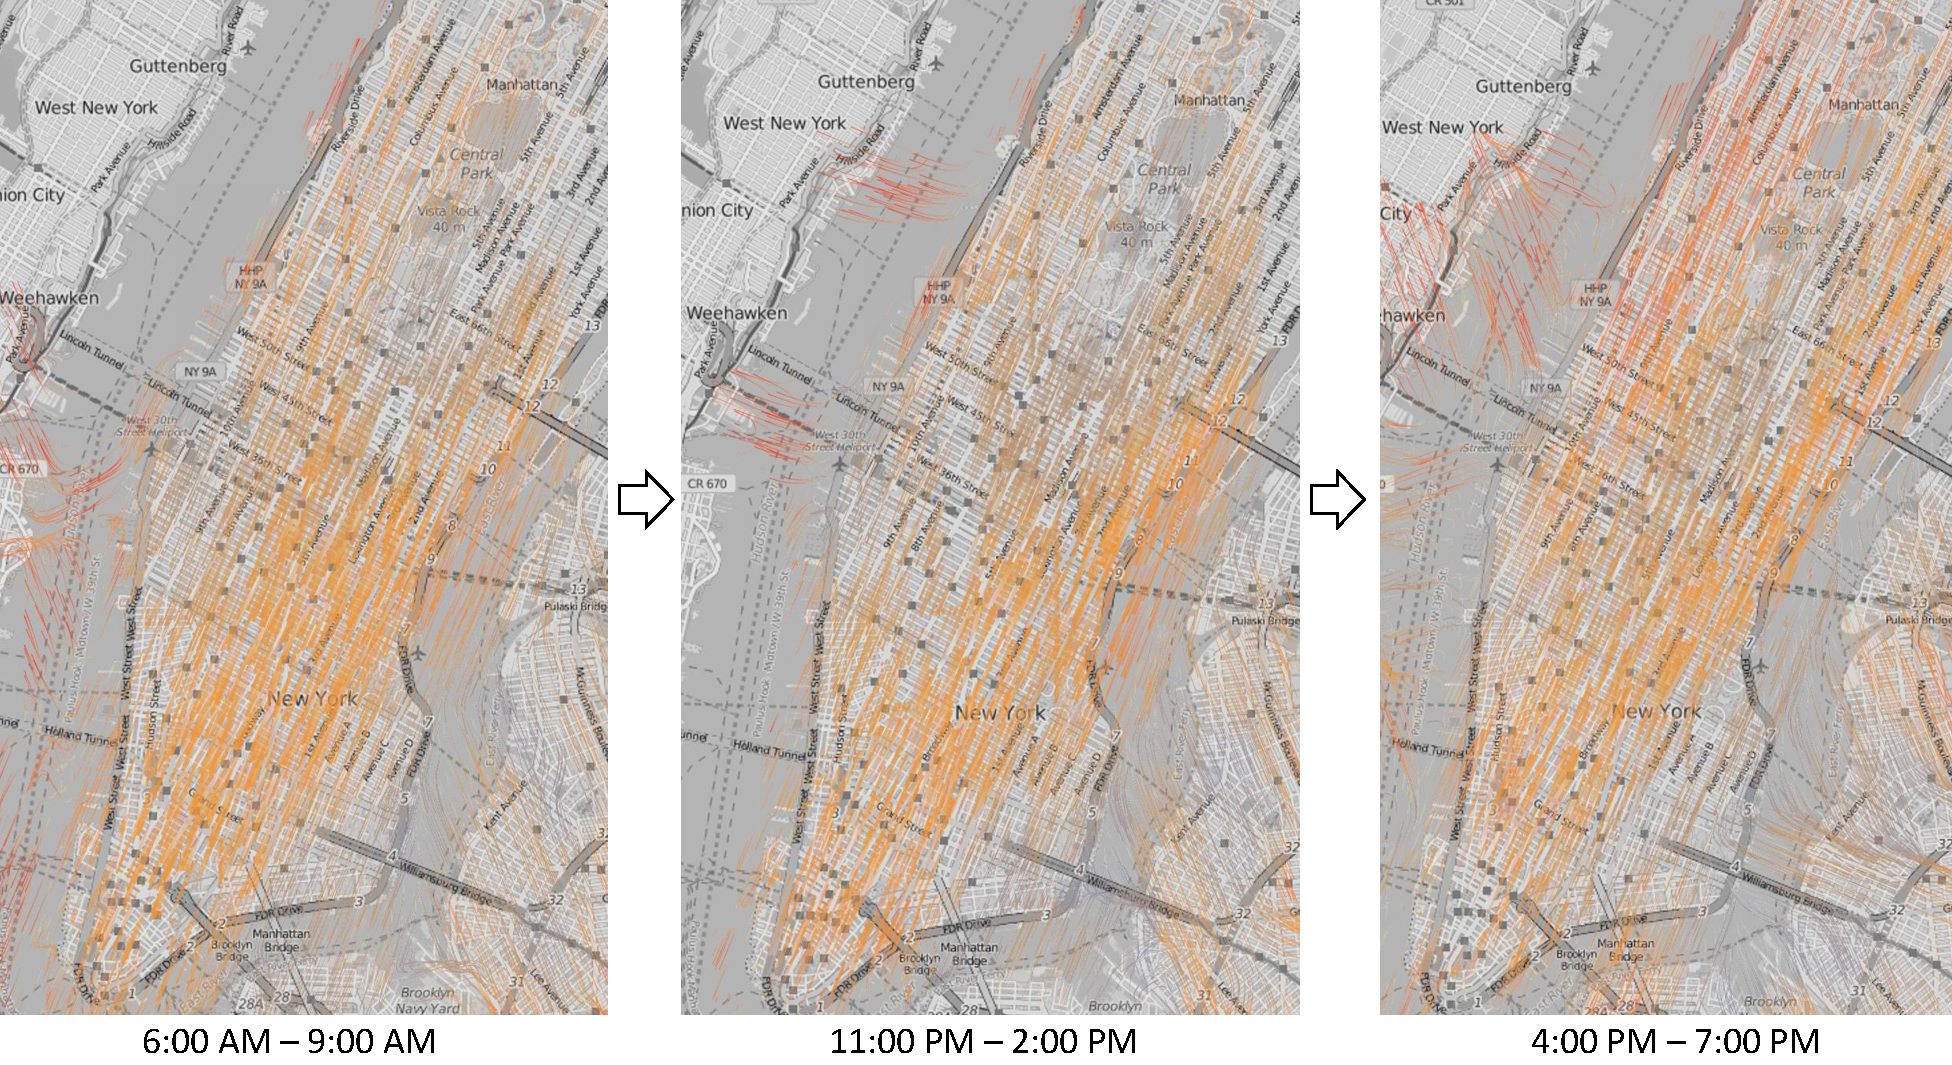
\includegraphics[width=1.0\linewidth]{case_study}
	\caption{The taxi flows of multiple different time frames in a day in Manhattan. It shows the major flow of taxi data during 6:00 AM – 9:00 AM (Left), 11:00 PM – 2:00 PM (Middle), and 4:00 PM – 7:00 PM (Right) on May 30, 2013.}
	\label{fig:case_study_taxi}
	%\vspace{-0.7cm}
\end{figure*} 


In Section~\ref{sec:discretization}, we introduce the directional density estimation to preserve the original vector directions instead of one dominant or average direction. Each direction has a density giving a hint for the probability of moving toward the direction. Since 8 sectors is set in each grid cell for the directions in this work, the densities for the 8 directions can be normalized and used as a probability. Moreover, a direction with high probability indicates that a flow is moving toward the direction with certainty, whereas, a flow moving to a direction with low probability becomes the uncertain flow. 

In order to represent the multi-vector fields in our flow visualization, particles are generated in the space and animated through the vector fields. The particle color is determined by the probability of the movement direction of the particle, where the color varies from the red to the blue gradually. The red indicates a high probability, whereas, the blue represents a low probability. Since the color is probability based, we can say that the red particle paths are more certain and the blue particle paths are relatively uncertain. In addition, since the number of samples utilized to compute the multi-vector field vary over the space, the number of samples are encoded as the intensity of the vector field. We visualize the intensity information in the width of the particle path (i.e., the wider paths indicate a larger group movement). For the vector directions, we animate the particles and fade out the tails to stress the current positions of the particles. 

Our system provides two different visualization modes for the multi-vector fields. One is a major flow and the other is a probability flow. The major flow is obtained by moving the particles toward the highest probability direction within a grid cell and the paths are colored with the highest probability within the cell. An example of the major flow is presented in Figure~\ref{fig:twitter_flow}~(A). Since each grid cell has only one possible direction, the flow fields are relatively smooth. Note that all colors are interpolated along the paths so that there is not abrupt color change. 

On the other hand, the probability flow is created based on the probabilities in the multi-vector field. Particles are randomly generated in the space and they move toward all non-zero directions in the multi-vector field. The number of particles in a given direction is proportional to the probability. For example, if there are two non-zero vectors (90\% and 10\%) in the multi-vector field and 100 particles are passing through the grid cell, 90 particles move in the 90\% vector direction, whereas, 10 particles move in 10\% vector direction. In addition, when a particle enters a new cell, the probability of the particle path is multiplied by the previous probability. In this way, we can compute all probabilities along the particle path from its birth to the death. The probability of each path segment is encoded in the path color as mentioned above. An example of probability flow is shown in Figure~\ref{fig:twitter_flow}~(B). Since the particle path is obtained by using multi-vector fields, the probability flow tends to become complex as all combinations of the flow directions between grid cells are visualized at the same time. Nonetheless, the color represents the certainty/uncertainty of the flow based on the probability of the path segment. Note that the width of the path segment represents the intensity of the vector field, which is proportional to the number of samples toward the direction as mentioned above. 



